\section{Resultados}

El primer experimento se realiz\'o utilizando el \\href{http://snap.stanford.edu/data/web-BerkStan.html}{Berkeley-Stanford web graph}. La cantidad de nodos/p\'aginas web es de 685230 y la cantidad de ejes/links es de 7600595.
Las pruebas se corrieron en una Intel Core i5-3550 CPU @ 3.30GHz x 4 con 8 GB de ram. 

\subsection{Propagaci\'on del error}

El experimento fue realizado variando la constante c, la cual determina la importancia proporcional que se quiere
entre la probabilidad de pasar a una p\'agina desde un link (c mas alto) contra la de escribir la url a mano (c mas bajo).

Como criterio de parada, comparamos la diferencia en norma uno del autovector que se obtiene
en cada iteraci\'on, contra el de la iteraci\'on anterior, la cual no debe ser menor que un
epsilon de orden -8.

A continuación mostramos, para distintos c, la cantidad de iteraciones que necesita el método de la potencia para alcanzar dicho epsilon, sin utilizar extrapolaci\'on cuadr\'atica primero, e incluy\'endola despu\'es:

\begin{figure}[H]
  \centering
    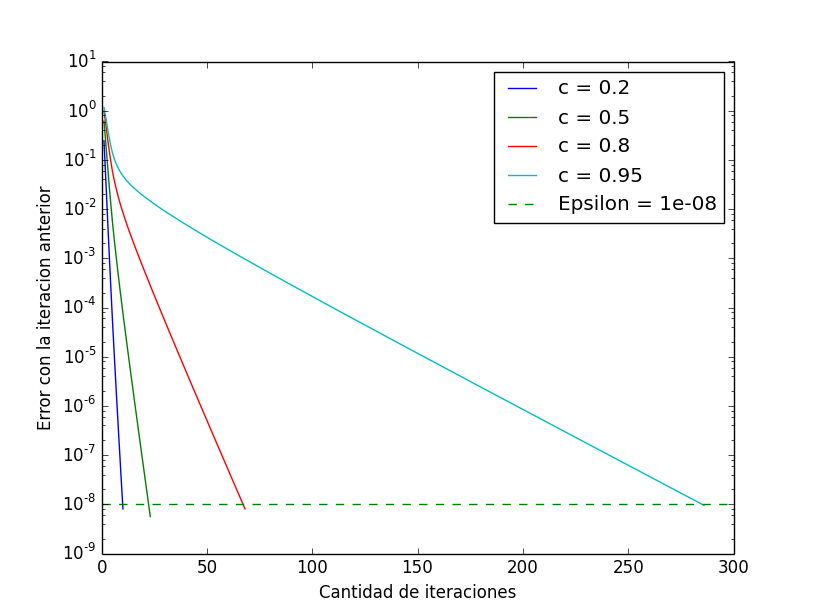
\includegraphics[width=0.9\textwidth]{errorSinQE.png}
    \caption{Error sin QE}
    \label{}
\end{figure}

\begin{figure}[H]
  \centering
    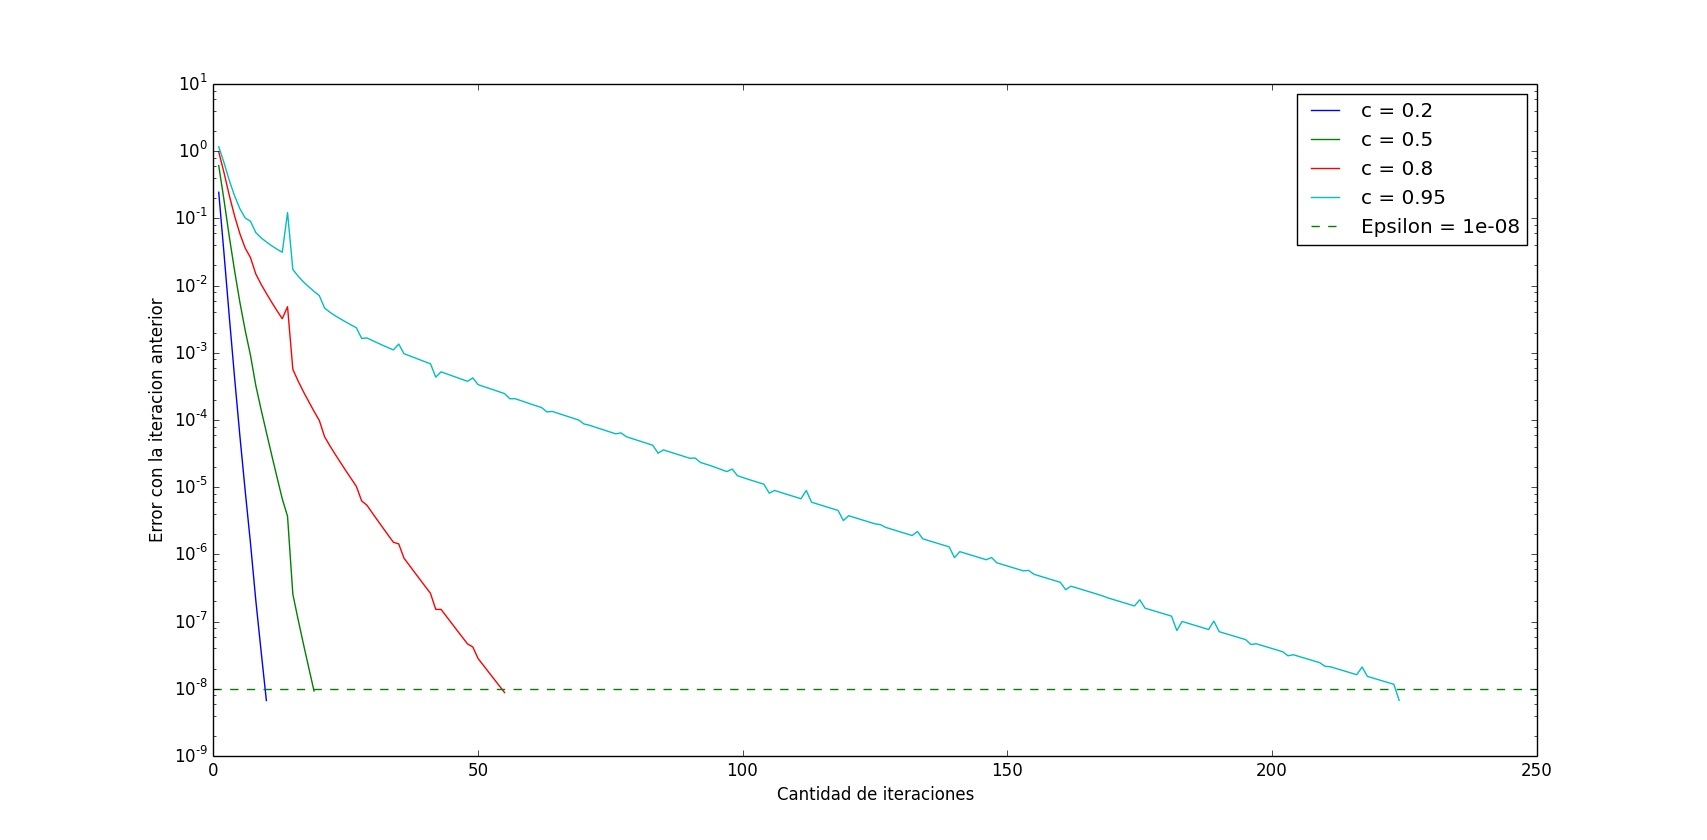
\includegraphics[width=0.9\textwidth]{errorConQE.png}
    \caption{Error con QE}
    \label{}
\end{figure}

El m\'etodo de extrapolaci\'on se aplica cada 7 iteraciones, en el gr\'afico anterior se puede ver que se presentan picos m\'inimos y m\'aximos, \'esto se debe a que el m\'etodo previamente nombrado cambia la diferencia entre los autovectores que se van calculando, pero luego ayuda a disminuir el error considerablemente.

Se puede obvservar en las figuras que cuanto menor es el c, m\'as r\'apido converge
el m\'etodo. Creemos que dicho resultado se debe a que al darle menor importancia
a los links directos, la matriz de probabilidades se encuentra mejor balanceada, 
por lo tanto los primeros autovalores de ella son mas parecidos y por ello se necesitan
m\'as iteraciones para lograr la convergencia.\\

La diferencia que se da al utilizar extrapolaci\'on no se ve f\'acilmente en los gr\'aficos anteriores, por lo que vamos a mostrarlo con mas detalle:

\begin{figure}[H]
  \centering
    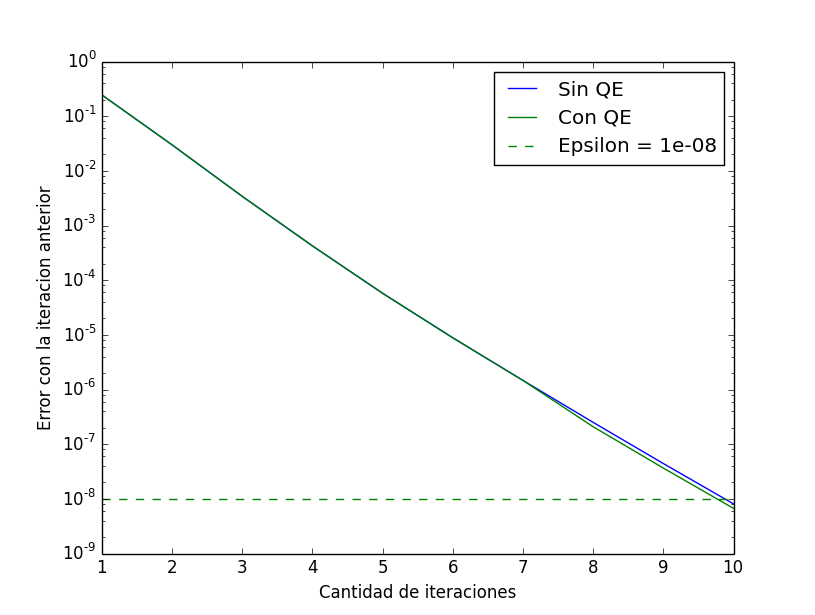
\includegraphics[width=0.8\textwidth]{comparando2.png}
    \caption{Comparaci\'on uso de QE con c = 0.2}
    \label{}
\end{figure}

\begin{figure}[H]
  \centering
    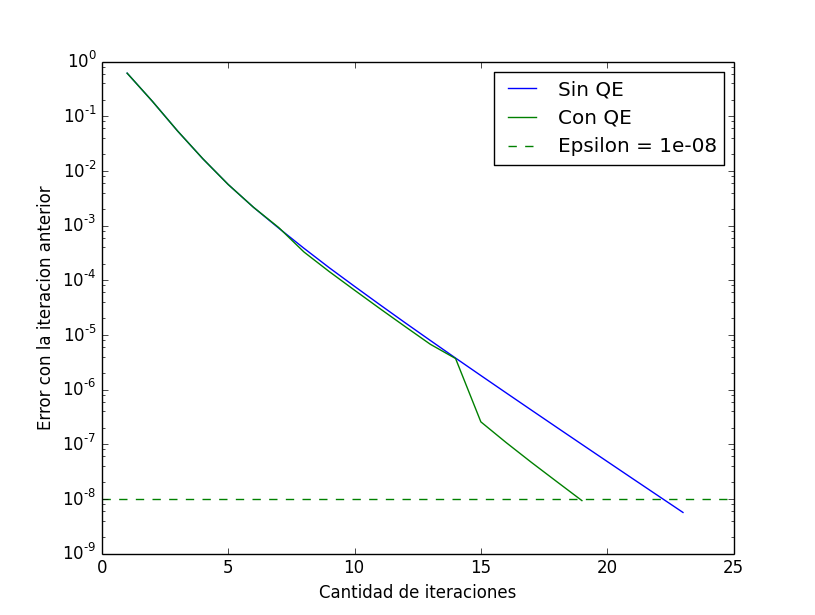
\includegraphics[width=0.8\textwidth]{comparando5.png}
    \caption{Comparaci\'on uso de QE con c = 0.5}
    \label{}
\end{figure}

\begin{figure}[H]
  \centering
    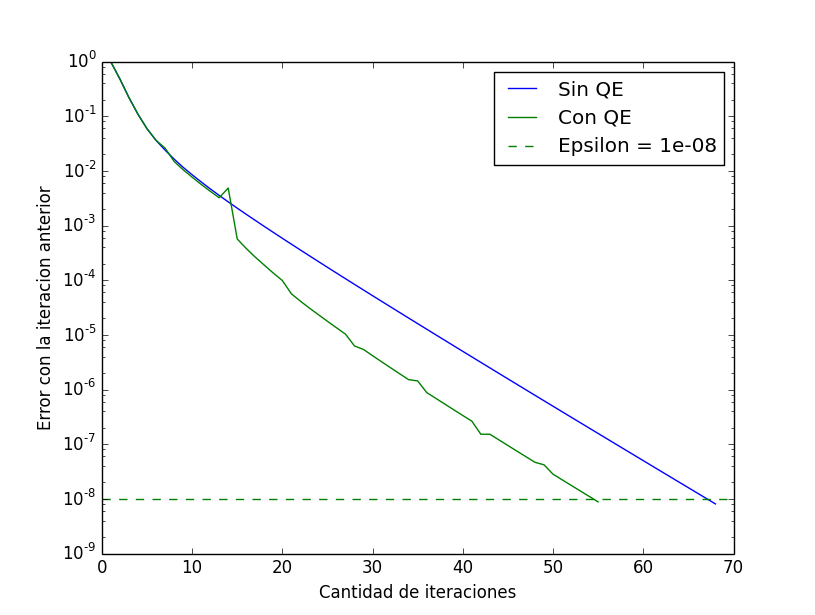
\includegraphics[width=0.8\textwidth]{comparando8.png}
    \caption{Comparaci\'on uso de QE con c = 0.8}
    \label{}
\end{figure}

\begin{figure}[H]
  \centering
    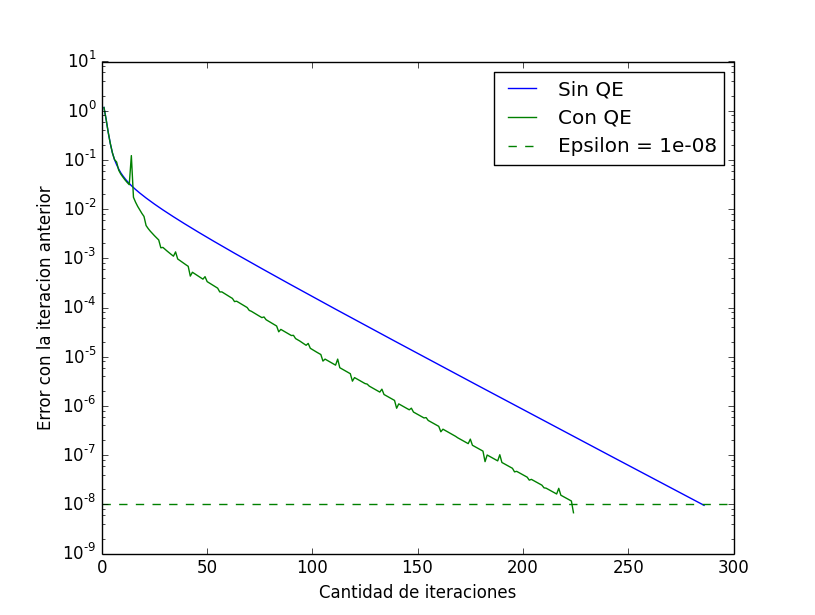
\includegraphics[width=0.8\textwidth]{comparando95.png}
    \caption{Comparaci\'on uso de QE con c = 0.95}
    \label{}
\end{figure}

En los gr\'aficos anteriores se nota la gran diferencia que hay cuando se aplica el m\'etodo de extrapolaci\'on cuadr\'atica, el cu\'al parece aumentar el error al principio, pero luego converge m\'as r\'apidamente. La diferencia tal vez no se aprecia tanto si la convergencia es muy r\'apida, como en el primer gr\'afico donde c es igual a 0.2, pero a medida que aumenta la cantidad de iteraciones, mas conveniente es utilizarlo.\\


\subsection{Tiempo de ejecuci\'on}

En cuanto a los tiempos de ejecuci\'on, notamos, que a pesar de la cantidad de iteraciones utilizando QE es menor, el m\'etodo de la potencia sin QE converge en menos tiempo de procesamiento (aunqe despreciable), pensamos que \'esto se puede deber a la falta de optimizaci\'on de c\'odigo por ejemplo, sin embargo, lo que nos interesa en mayor medida es la cantidad de iteraciones necesarias, donde como ya vimos, QE es el claro vencedor. 
\'Estos fueron los resultados arrojados por el algoritmo: \\

\begin{tabular}{ l | c | r}
  & Sin QE & Con QE\\
  \hline
  c = 0.2 & 2 segs. & 3 segs.\\
  \hline
  c = 0.5 & 6 segs. & 5 segs.\\
  \hline
  c = 0.8 & 15 segs. & 16 segs. \\
  \hline
  c = 0.95 & 65 segs. & 69 segs. \\
  \hline
\end{tabular}


\subsection{Relevancia de las p\'aginas}

\begin{table}\begin{center}
\subfloat[][Rank obtenido con $c = 0.2$]{\begin{tabular}{ l | c }
  \hline
www.ole.com.ar & 0.0484629 \\
www.clarin.com & 0.0468603 \\
www.ciudad.com.ar & 0.0430782 \\
www.clasificados.clarin.com & 0.0430782 \\
www.youtube.com & 0.0420166 \\
www.taringa.net & 0.0420166 \\
canchallena.lanacion.com.ar & 0.0418644 \\
www.lanacion.com.ar & 0.0418644 \\
www.zonaprop.com.ar & 0.0405957 \\
www.rollingstone.com.ar & 0.0405957 \\
maps.google.com.ar & 0.0385152 \\
www.twitter.com & 0.0385152 \\
www.clarin.com/deportes & 0.0373568 \\
www.9gag.com & 0.0350138 \\
www.stackoverflow.com & 0.0350138 \\
www.facebook.com & 0.0350138 \\
www.hotmail.com & 0.0350138 \\
www.gmail.com & 0.0350138 \\
www.assembla.com & 0.0350138 \\
www.github.com & 0.0350138 \\
www.mercadolibre.com.ar & 0.0350138 \\
www.yahoo.com & 0.0350138 \\
www.pagina12.com.ar & 0.0350138 \\
www.mamapuntocero.com.ar & 0.0350138 \\
www.infobae.com & 0.0350138 \\
www.google.com & 0.0350138 \\
  \hline
\end{tabular}
}
\qquad
\subfloat[][Rank obtenido con $c = 0.5$]{
\begin{tabular}{ l | c }
  \hline
www.ole.com.ar & 0.0708548 \\
www.clarin.com & 0.0679806 \\
www.ciudad.com.ar & 0.0551093 \\
www.clasificados.clarin.com & 0.0551093 \\
canchallena.lanacion.com.ar & 0.0476948 \\
www.lanacion.com.ar/ & 0.0476948 \\
www.zonaprop.com.ar & 0.0445151 \\
www.rollingstone.com.ar & 0.0445151 \\
www.youtube.com & 0.0429253 \\
www.taringa.net & 0.0429253 \\
www.clarin.com/deportes & 0.0371144 \\
maps.google.com.ar & 0.0357711 \\
www.twitter.com & 0.0357711 \\
www.9gag.com & 0.0286169 \\
www.stackoverflow.com & 0.0286169 \\
www.facebook.com & 0.0286169 \\
www.hotmail.com & 0.0286169 \\
www.gmail.com & 0.0286169 \\
www.assembla.com & 0.0286169 \\
www.github.com & 0.0286169 \\
www.mercadolibre.com.ar & 0.0286169 \\
www.yahoo.com & 0.0286169 \\
www.pagina12.com.ar & 0.0286169 \\
www.mamapuntocero.com.ar & 0.0286169 \\
www.infobae.com & 0.0286169 \\
www.google.com & 0.0286169 \\
\hline
\end{tabular}
}
\\ 
\vspace{0.5cm}
\subfloat[][Rank obtenido con $c = 0.8$]{\begin{tabular}{ l | c }
  \hline
www.ole.com.ar & 0.122585 \\
www.clarin.com & 0.119996 \\
www.ciudad.com.ar & 0.0862634 \\
www.clasificados.clarin.com & 0.0862634 \\
canchallena.lanacion.com.ar & 0.0492588 \\
www.lanacion.com.ar/ & 0.0492588 \\
www.zonaprop.com.ar & 0.0445675 \\
www.rollingstone.com.ar & 0.0445675 \\
www.clarin.com/deportes & 0.0422953 \\
www.youtube.com & 0.032933 \\
www.taringa.net & 0.032933 \\
maps.google.com.ar & 0.0256146 \\
www.twitter.com & 0.0256146 \\
www.9gag.com & 0.0182961 \\
www.stackoverflow.com & 0.0182961 \\
www.facebook.com & 0.0182961 \\
www.hotmail.com & 0.0182961 \\
www.gmail.com & 0.0182961 \\
www.assembla.com & 0.0182961 \\
www.github.com & 0.0182961 \\
www.mercadolibre.com.ar & 0.0182961 \\
www.yahoo.com & 0.0182961 \\
www.pagina12.com.ar & 0.0182961 \\
www.mamapuntocero.com.ar & 0.0182961 \\
www.infobae.com & 0.0182961 \\
www.google.com & 0.0182961 \\
  \hline
\end{tabular}
}
\qquad
\subfloat[][Rank obtenido con $c = 0.95$]{
\begin{tabular}{ l | c }
  \hline
www.ole.com.ar & 0.205635 \\
www.clarin.com & 0.204461 \\
www.ciudad.com.ar & 0.138847 \\
www.clasificados.clarin.com & 0.138847 \\
www.clarin.com/deportes & 0.0559973 \\
canchallena.lanacion.com.ar & 0.028682 \\
www.lanacion.com.ar/ & 0.028682 \\
www.zonaprop.com.ar & 0.0256032 \\
www.rollingstone.com.ar & 0.0256032 \\
www.youtube.com & 0.0145039 \\
www.taringa.net & 0.0145039 \\
maps.google.com.ar & 0.0109709 \\
www.twitter.com & 0.0109709 \\
www.9gag.com & 0.00743788 \\
www.stackoverflow.com & 0.00743788 \\
www.facebook.com & 0.00743788 \\
www.hotmail.com & 0.00743788 \\
www.gmail.com & 0.00743788 \\
www.assembla.com & 0.00743788 \\
www.github.com & 0.00743788 \\
www.mercadolibre.com.ar & 0.00743788 \\
www.yahoo.com & 0.00743788 \\
www.pagina12.com.ar & 0.00743788 \\
www.mamapuntocero.com.ar & 0.00743788 \\
www.infobae.com & 0.00743788 \\
www.google.com & 0.00743788 \\
\hline
\end{tabular}
}

\caption{Rank obtenido para distintos valores de $c$}
\end{center}\end{table}

Tal como esper\'abamos ver, las 15 p\'aginas que antes hab\'iamos notado que no ten\'ian links entrantes, son las \'ultimas
en la tabla, y no casualmente, tienen todas la misma relevancia.

Otra cosa que notamos al ir aumentando el c es que, dejando de lados los cambios en el orden de la tabla (que eran menores),
los n\'umeros cada vez se parec\'ian m\'as, ya que al darle mas importancia a las url que a los links, la cantidad
de links de entrada que posee una p\'agina no entra tanto en juego y todas se consideran iguales en t\'erminos de relevancia.
